\documentclass[12pt]{article}

\usepackage{fontawesome}
\usepackage{hyperref}
\usepackage{xurl}
\usepackage{fancyvrb}
\usepackage{graphicx}
\usepackage{float}
\usepackage[tagged, highstructure]{accessibility}
\usepackage{bookmark}
\usepackage{enumitem}

\hypersetup{
    colorlinks=false,
    pdfborder={0 0 0},
    pdftitle={Beyond SQL},
    pdfauthor={Adrianna Holden-Gouveia},
    pdfsubject={Advanced Data - Lab Assignment},
    pdflang={en-US},
    pdfkeywords={database implementation, relational database, non-relational, SQLite}
}

% Configure PDF bookmarks for navigation
\bookmarksetup{
    numbered,
    open,
}

% Configure list spacing for better accessibility
\setlist{nosep}



\title{Beyond SQL}
\author{
        Adrianna Holden-Gouveia \\
        Website: \href{https://aholdengouveia.name}{aholdengouveia.name}\\ 
        \date{\vspace{-5ex}}
        %Email: \href{mailto:admin@aholdengouveia.name}{admin@aholdengouveia.name} \\
%        \faLinkedin{: aholdengouveia} \\
        \faGithub {: aholdengouveia} \\
        %\faTwitter {: aholdengouveia} \\
        }

%S\date{\today}


\begin{document}    

\maketitle

%\begin{abstract}
%This is a template for Linux Administration Lab work
%\end{abstract}
%\tableofcontents


\section*{Accessibility Notice}
This document is also available in HTML format at:

Link: \href{https://aholdengouveia.name/AdvData/labs/week8beyondSQL.html}{\textbf{\nolinkurl{https://aholdengouveia.name/AdvData/labs/week8beyondSQL.html}}}

The HTML version provides enhanced accessibility features including keyboard navigation, screen reader support, responsive design, dark mode support, and high contrast options.

\section*{Request}
\noindent\textbf{Request:} DATA-9025\\
\textbf{Requested by:} Head of the data team\\
\textbf{Data:} Your database from the SQL Review lab, and your schema from the Database Schema lab

\section*{Background}
Your design has been approved, so now it's time to build it. Your manager wants your data moved out of the one big table and into the tables in your schema, cleaned up along the way, with a record of every change. The team is also starting to look at other kinds of databases, so your manager wants a quick comparison of relational and non-relational databases for your data.

\section*{Learning Outcomes}
By the end of this lab, you will be able to:
\begin{itemize}
    \item Organize a data set into multiple tables based on a schema, and load it into a database
    \item Clean up data, and record each change in a cleanup log
    \item Decide which ways to reduce repeated data to use, and justify each decision with research
    \item Compare relational and non-relational databases for a data set
\end{itemize}

\section*{Lab Instructions}
Start from the database you turned in for the SQL Review lab, and add your lookup table from the SQL Review Part 2 lab if it's part of your schema. Books are my example data only, so use your own data set. If you want to switch to a different data set, email me first. Switching means redoing the work from earlier labs for your new data set, so it adds a lot of work. The switching checklist (linked under Resources) lists what you'd need to redo.

I suggest SandboxSQL, linked under Resources. Use Load a Database to open the database file you turned in for the SQL Review lab. You can use a different tool if you prefer, as long as you turn in a database file, not a CSV file or a spreadsheet. SandboxSQL doesn't always keep your work if you close the page, so export often. If you need to load your raw data again, use my CSV to Database Converter (linked under Resources).

Name your files with version numbers, such as version 1.0 and 2.0 for big changes, and 1.1 and 1.2 for small ones (for example, Database1.1). Don't use names like Database Final and Database Final REALLY final.

\subsection*{Screenshots}
Several parts of this lab ask for a screenshot. Each screenshot should have your name, term, and year.  One of the easiest ways to do that is make a text document with your name and term/year on your computer and save it to use all term. Any screenshots that don't include this information won't be counted.

\begin{figure}[H]
    \centerline{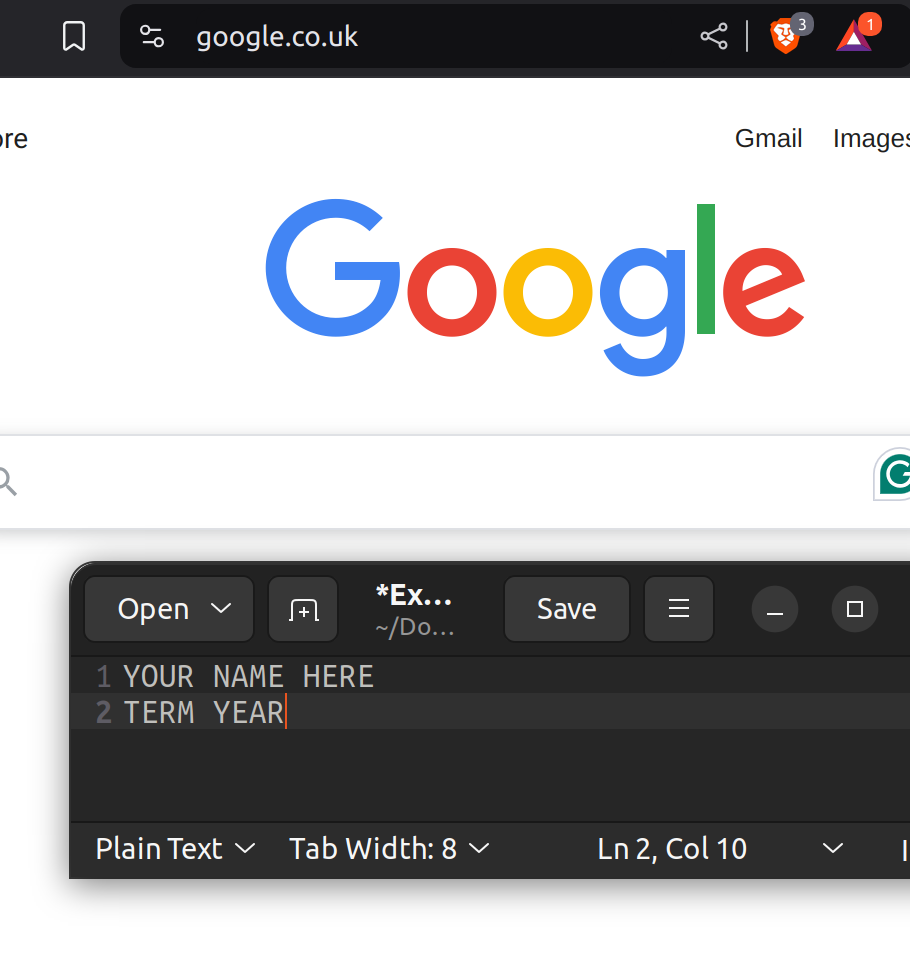
\includegraphics[scale=.2]{ExampleScreenshot.png}}
    \caption{This is an image of what each of your screenshots should look like}
    \alt{Example screenshot: a web browser showing the Google home page, with a small text editor window in front of it that says YOUR NAME HERE and TERM YEAR}
\end{figure}

\subsection*{Part 1: Decide How to Reduce Repeated Data}
In the Database Schema lab, you made at least 2 suggestions for reducing repeated data.
\begin{enumerate}
    \item For each suggestion, decide whether to use it now, save it for later, or not use it at all.
    \item Research each decision, using at least 2 reliable sources in total. Check each source with the CRAAP test (linked under Resources), and cite each one with a link.
    \item Explain each decision in a few sentences, using your research.
    \item If your decisions change your schema, update it. Put anything new or changed in bold, and add a short note saying what changed and why.
\end{enumerate}

\subsection*{Part 2: Build Your Tables}
\begin{enumerate}
    \item Create each table in your schema, with its primary key and any foreign keys.
    \item Copy your data from your one big table into the new tables. One way is INSERT with SELECT. For example, this fills a publishers table with one row for each different publisher in my book data:
\begin{Verbatim}
INSERT INTO publishers (publisher_name)
SELECT DISTINCT publisher FROM books;
\end{Verbatim}
    The SQLite documentation for INSERT is linked under Resources.
    \item Keep your original big table until everything is copied over and checked. Then you can delete it, or keep it as a copy of the raw data.
    \item Take a screenshot of your database structure showing all your tables, and a screenshot of one of your new tables with data in it.
\end{enumerate}

\subsection*{Part 3: Clean Up Your Data}
Fix the problems you listed in the quality notes on your data card, and any others you find. Record every fix in a cleanup log, following the sample cleanup log (linked under Resources). For each entry, give the date, whether it was before, during, or after loading, the table and column, the problem, the change you made, why, and how many rows were affected. If you checked something and decided not to change it, log that too.

\subsection*{Part 4: Export Your Database}
\begin{enumerate}
    \item Export your whole database as a file. In SandboxSQL, use the Export button, which saves it as a .sqlite file.
    \item Run this query, which lists the CREATE TABLE command for every table in your database:
\begin{Verbatim}
SELECT name, sql FROM sqlite_master WHERE type = 'table';
\end{Verbatim}
    Take a screenshot of the results.
    \item Pick one CREATE TABLE command, and explain in your own words what each part of it does, including the keys.
\end{enumerate}

\subsection*{Part 5: Relational or Non-Relational?}
Make a pro and con list or table for keeping your data in a relational database, and for moving it to a non-relational database. Give at least 3 pros and 3 cons for each, specific to your data.

\section*{Acceptance Criteria}
This request is done when:
\begin{itemize}
    \item Every suggestion from the Database Schema lab has a decision, backed by research from at least 2 cited sources that you've checked with the CRAAP test
    \item Every table in your schema exists in your database, with its primary key and any foreign keys
    \item Your data is in the new tables, and your screenshots show the tables and data
    \item Every change to your data is in your cleanup log, including the number of rows affected
    \item Your exported database includes all your tables, and you've explained one CREATE TABLE command
    \item At least 3 pros and 3 cons each for relational and non-relational, specific to your data
    \item Every screenshot follows the screenshot rules
\end{itemize}

\section*{Deliverables}
Two files:
\begin{enumerate}
    \item A document that includes Part 1, your decisions, research, and any schema changes; Part 2, your screenshots; Part 3, your cleanup log; Part 4, your screenshot and your explanation of one CREATE TABLE command; and Part 5, your pros and cons
    \item Your exported database file
\end{enumerate}

Audience: the head of the data team.

\section*{Resources}
References, a video, a PowerPoint and some notes are available at my website
Link: \href{https://www.aholdengouveia.name/AdvData/BeyondSQL.html}{\textbf{\nolinkurl{https://www.aholdengouveia.name/AdvData/BeyondSQL.html}}}

Sample cleanup log, showing the format to follow
Link: \href{https://www.aholdengouveia.name/AdvData/labs/SampleCleanupLog.txt}{\textbf{\nolinkurl{https://www.aholdengouveia.name/AdvData/labs/SampleCleanupLog.txt}}}

SQLite documentation for INSERT
Link: \href{https://www.sqlite.org/lang_insert.html}{\textbf{\nolinkurl{https://www.sqlite.org/lang_insert.html}}}

My CSV to Database Converter, which makes a database file from your CSV file
Link: \href{https://www.aholdengouveia.name/AdvData/labs/csv-to-database.html}{\textbf{\nolinkurl{https://www.aholdengouveia.name/AdvData/labs/csv-to-database.html}}}

Suggested tool: SandboxSQL, free, runs in your browser, and saves your database as a .sqlite file with its Export button
Link: \href{https://www.sandboxsql.com/}{\textbf{\nolinkurl{https://www.sandboxsql.com/}}}

Optional, if you'd rather install a tool: DB Browser for SQLite, which can import a CSV file directly
Link: \href{https://sqlitebrowser.org/}{\textbf{\nolinkurl{https://sqlitebrowser.org/}}}

The CRAAP test, for checking your sources
Link: \href{https://web.archive.org/web/20250814000638/https://guides.lib.uchicago.edu/c.php?g=1241077&p=9082343}{\textbf{\nolinkurl{https://web.archive.org/web/20250814000638/https://guides.lib.uchicago.edu/c.php?g=1241077&p=9082343}}}

My guide to evaluating sources
Link: \href{https://www.aholdengouveia.name/Howtos/Sourceeval/sourceEvaluation.html}{\textbf{\nolinkurl{https://www.aholdengouveia.name/Howtos/Sourceeval/sourceEvaluation.html}}}

Switching checklist, if you want to change data sets
Link: \href{https://www.aholdengouveia.name/AdvData/labs/SwitchingDataSets.txt}{\textbf{\nolinkurl{https://www.aholdengouveia.name/AdvData/labs/SwitchingDataSets.txt}}}

\end{document}